\documentclass{beamer}
%
% Choose how your presentation looks.
%
% For more themes, color themes and font themes, see:
% http://deic.uab.es/~iblanes/beamer_gallery/index_by_theme.html
%
\mode<presentation>
{
  \usetheme{default}      % or try Darmstadt, Madrid, Warsaw, ...
  \usecolortheme{default} % or try albatross, beaver, crane, ...
  \usefonttheme{default}  % or try serif, structurebold, ...
  \setbeamertemplate{navigation symbols}{}
  \setbeamertemplate{caption}[numbered]
} 

\usepackage[english]{babel}
\usepackage[utf8x]{inputenc}
\usepackage[font=small]{caption}
\graphicspath{ {./img/} }

\title[PR1/2 Demo]{PR1/2 Demo}
\author{Christian Permann}
\institute{Faculty of Computer Science, University of Vienna,\newline W\"ahringer Stra{\ss}e 29, 1090 Vienna}
\date{13.11.2018}

\begin{document}

\begin{frame}
  \titlepage
\end{frame}

% Uncomment these lines for an automatically generated outline.
%\begin{frame}{Outline}
%  \tableofcontents
%\end{frame}

\section{Current Progress}

\begin{frame}{Milestones P1 updated}

\begin{itemize}
  \item Create a basic visualization tool. (done)
  \item Define interface for data manipulation. (done)
  \item (Be compatible with ELKI.)
  \item Allow data import. (CSV/Arff available, done)
  \item Create data generation logic. (ELKI generator available, possibly add simple GUI with reduced functionality)
  \item Create dim-reduction for visualization and implement it. (PCA and T-SNE, done)
  \item Allow to generate a scatter plot matrix. (done)

\end{itemize}

\end{frame}

\section{Tool}

\begin{frame}{The Tool}

\centerline{Demo}

\end{frame}

\begin{frame}{The Tool - Dimensionality Reduction Interface}
\begin{center}
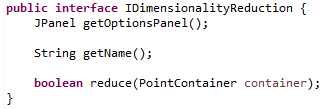
\includegraphics[width=0.7\textwidth]{interface}
\end{center}
\captionof{figure}{The interface for dimensionality reduction}

\end{frame}

\section{Papers}

\begin{frame}{Papers for PR2}

\begin{itemize}
  \item LineUp: Visual Analysis of Multi-Attribute Rankings \cite{2013_infovis_lineup}
  \item WeightLifter: Visual Weight Space Exploration for Multi-Criteria Decision Making \cite{cs4804}
  \item Metric Factorization for Exploratory Analysis of Complex Data \cite{7023368}
  \item DimStiller: Workflows for dimensional analysis and reduction \cite{cs4209}
  \item Comparing clusterings: an axiomatic view \cite{Meila05comparingclusterings:}
  \item Comparing subspace clusterings \cite{1637417}
  \item External evaluation measures for subspace clustering \cite{Gunnemann:2011:EEM:2063576.2063774}
\end{itemize}

\end{frame}

\section{Ideas}

\begin{frame}{Ideas for evaluating Clusterings}
\begin{itemize}
\item different quality measures as described in \cite{Gunnemann:2011:EEM:2063576.2063774}
\item a weighted average of measures like in ClusterVision\cite{8019866}
\item using \cite{2013_infovis_lineup,cs4804,7023368} as basis for analyzing the quality of measures and deciding on different weights (kind of a better reasoning for the choice compared to clustervision)
\item \textbf{clustering (OPTICS?) clusterings and visualizing groups of results across multiple algorithms and settings (new idea?) using \cite{Meila05comparingclusterings:,1637417}} in regards to the distance measure
\item possibly training a weighted average of measures via supervision with a Neural Network (needs lots of data and known optimal clusterings; generalizeable result?)

\end{itemize}
\end{frame}

\section{Cluster Clustering}

\begin{frame}{My Idea}

Using OPTICS to cluster clusterings could result in a reachability plot that hierarchically shows groups of clustering results that agree on the result. The output of the algorithm can also be visualized in a symmetric heat-map as shown in our OPTICSVis Project. Here it may be possible to see which clusterings overlap with others and which are vastly different, in a hierarchical view. One problem here may be though, that the distance measure should satisfy the triangle inequality for useful measures(, I think). (see Figure \ref{clusteringError}: Clustering Error Metric)

\end{frame}


\begin{frame}{Distance Measure}

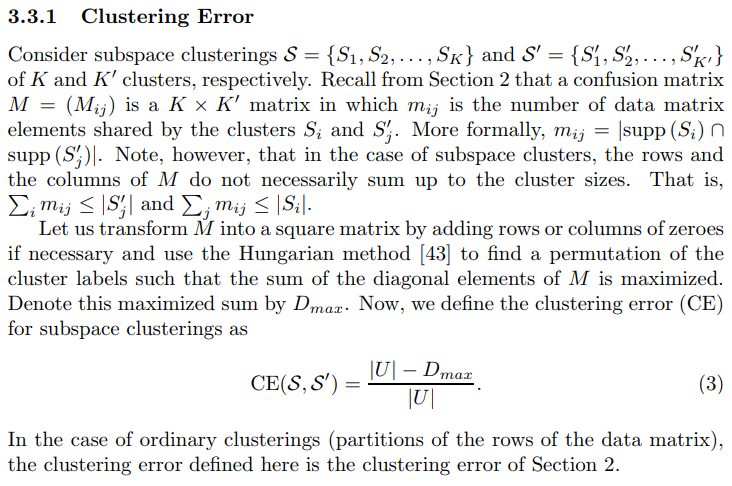
\includegraphics[width=\textwidth]{ClusteringError}
\captionof{figure}{Distance Measure from \cite{1637417}}
\label{clusteringError}
\end{frame}


\bibliography{citations}
\bibliographystyle{ieeetr}

\end{document}